\newcommand{\Normal}{\mathrm{Normal}}
\newcommand{\Borel}{\mathcal{B}}
\newcommand{\Ex}{\mathbb{E}}

\begin{quote}
\textit{This branch of mathematics [Probability] is the only one, I believe, in which good writers frequently get results which are entirely erroneous.}

\hfill Charles S. Peirce
\end{quote}

\section{Introduction}

Probability is notorious for being counterintuitive.
Ask anyone who is wrestling with the birthday paradox, the Monty Hall problem, or the Bayesian phenomenon \emph{explaining away}.

Probability's habit of violating intuition makes any automation of probabilistic reasoning helpful.
In Bayesian statistics, automation has been taking the form of modeling languages for probabilistic processes.
The languages' implementations compute answers to questions about the processes under constraints.

Probabilistic languages should have mathematical specifications.
The reason is simple: if a probabilistic language is implemented to be faithful to its maker's intuitions instead of a specification, it is almost certainly faulty.

Unfortunately, there are currently few probabilistic languages that have mathematical specifications.
This state of affairs is partly responsible for another: until now, every probabilistic language that can support Bayesian practice is artificially limited in what it can express.
Most commonly, probabilistic languages disallow unbounded loops and recursion, allow only discrete or continuous distributions, and restrict constraints to the form $X = c$.

The thesis statement is essentially that these states of affairs need not continue.

\newpage

%\begin{quote}
%\textbf{Functional programming theory} and \textbf{measure-theoretic probability} provide a \textbf{solid foundation} for \textbf{trustworthy}, \textbf{useful} languages for \textbf{constructive probabilistic modeling} and \textbf{inference}.
%\end{quote}

\begin{quote}
\textbf{Thesis Statement:} Functional programming theory and measure-theoretic probability provide a solid foundation for trustworthy, useful languages for constructive probabilistic modeling and inference.
\end{quote}

\section{Terms}

To \keyword{model} something is to make it into a model of a theory, by developing the theory. For example, physicists model gravity by developing theories of gravitation; the physical phenomenon is a model of the theories. Likewise, Bayesians model probabilistic processes by developing probabilistic theories for which the physical processes are models.
When there are mathematical models of theories, the mathematical models can be used to predict the physical models' behavior and discover their properties.

Bayesians write theories in many ways. One is to write them \keyword{constructively}: in such a way that the theory contains enough information to directly construct one of its mathematical models. This is often regarded as the ideal way to write them.

\keyword{Inference} means answering questions about theories.
In this context, it implies \keyword{conditioning}: constraining the model in a way that preserves certain relative probabilities.

\keyword{Measure-theoretic probability}~\cite{cit:klenke-2006-probability} is the most successful theory of probability in precision, maturity, and explanatory power. It was first developed in the early 1900s to formalize intuitive ideas about probability, to unify notions of discrete and continuous random variables, and to settle paradoxes that arise from incorrectly applying intuition to infinities.

\keyword{Functional programming theory} is used to give mathematically precise meaning to programs and to give rules for executing them. In it, the $\lambda$-calculus serves as a model of computation and as a minimal language in which to reason by substitution.

A \keyword{trustworthy} language has a mathematical meaning called a \keyword{semantics}.
By defining a language mathematically, it is possible to prove theorems about it, which apply to all faithful implementations.
Further, if a language implementation computes something unexpected, its semantics provides a way to determine whether its behavior is correct.

We generally think of languages as being \keyword{useful} when they save time by automating calculations.
Languages are also useful when they allow us to express ideas naturally and reason about them precisely, or provide abstraction mechanisms so we can express ideas and reason about them at high levels.

\section{Proof and Supporting Evidence}

All but usefulness in the thesis can be proved, and for usefulness, we give evidence.
To prove and demonstrate the thesis, we define two semantics, prove them correct, implement approximations of them, and test the implementations.

The first semantics is an initial investigation into our general approach: transforming Bayesian theories into $\lambda$-calculus terms that build exact measure-theoretic models of the theories, and then changing the transformation to build approximate models to carry out computations.
To keep the investigation simple, we restrict theories to countable probability distributions and finitely many statements.

We ensure the first language is trustworthy by deriving its semantics from an idealized expected meaning of Bayesian theories, and computing answers to queries from approximate models in a way that converges to the correct answers according to the exact models.
We demonstrate the language is useful by implementing the approximating transformation, and encoding theories and running queries that are difficult to model directly without it.

The second semantics handles uncountable probability distributions and recursion by transforming a first-order functional language with probabilistic choice into $\lambda$-calculus terms that build models.
Again, we change the transformation to build approximate models and use them to carry out computations.

We show the language is trustworthy by proving
\begin{itemize}
	\item Exact queries always terminate with correct answers (Theorem~\ref{cor:correct-convergence}).
	\item All probabilistic programs have sensible output distributions, regardless of nontermination (Theorems~\ref{thm:proto-all-programs-measurable} and~\ref{thm:proto-all-projections-measurable}).
	\item The approximations are sound, always terminate, and have other desirable properties (Theorems~\ref{thm:terminating} through~\ref{thm:decreasing}).
	\item Answers computed using the approximations correctly converge (Theorem~\ref{thm:partitioned-importance-sampling-correctness}).
\end{itemize}
Further, Theorems~\ref{thm:proto-all-programs-measurable} and~\ref{thm:proto-all-projections-measurable} apply to any probabilistic programming language that can be transformed into ours.
Because ours is Turing-equivalent (with a random oracle) and is easy to extend with uncomputable operations such as real limits and decidable equality, this includes all probabilistic programming languages to date, and likely almost all future probabilistic programming languages.

We demonstrate the second language is useful by implementing the approximating transformation and encoding some typical Bayesian theories and running queries.
In all of our tests, the theory encodings are straightforward and the queries are efficient.

To demonstrate further usefulness, we encode theories and run queries that are impossible to reason about precisely using typical Bayesian mathematical tools.
One example draws inferences from a correctly modeled thermometer.
Another is a simple, direct theory of light transport and a query that together carry out stochastic ray tracing.

\section{Exposition Transition System}

While this work is designed to make sense when read straight through, readers may skip some depending on their goals.

\begin{figure*}[!tb]\centering
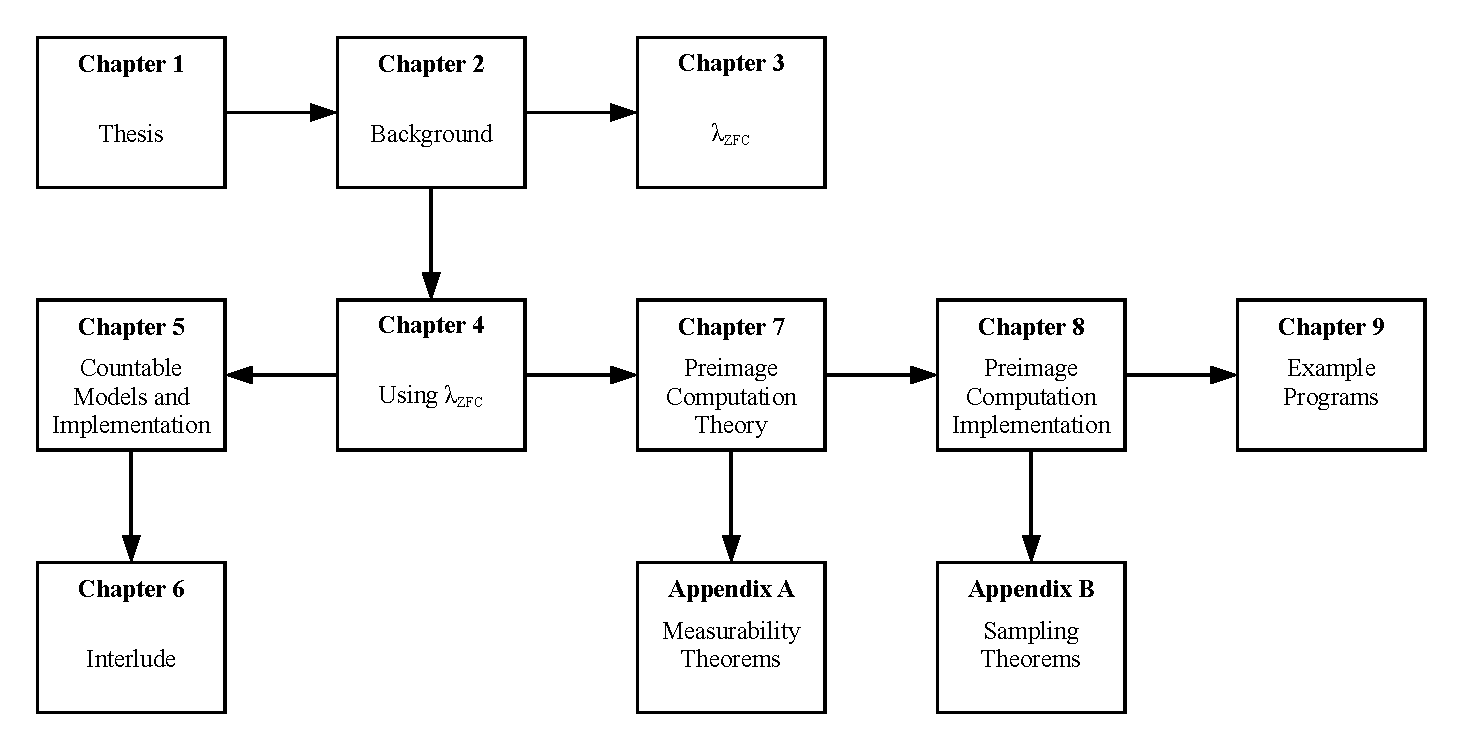
\includegraphics[width=\textwidth]{figures/reading-graph}
\caption[A transition system for reading this dissertation]{A transition system showing possible paths through this dissertation.}
\label{fig:reading-graph}
\end{figure*}

In principle, answers to questions such as ``Which chapters should I read if I am only interested in implementations of probabilistic languages with conditioning and recursion?'' can be answered using a dependency graph.
However, the graph would be a mess of arrows: for example, everything after Chapter~\ref{ch:background} (Background) depends on Chapter~\ref{ch:background}; similarly for Chapter~\ref{ch:using-lambda-zfc} (Using \lzfclang).
\figref{fig:reading-graph} shows an alternative: a transition system on chapters for which following any path (with backtracking permitted) guarantees a reader will not miss out on prerequisites.

Chapter~\ref{ch:background} gives the necessary background in Bayesian practice and functional programming theory, and motivates using measure theory.

The two semantics mentioned in the preceeding section transform programs into $\lambda$-calculus terms.
This target language has three requirements that are unusual for a $\lambda$-calculus: it must be able to represent infinite objects and operations on them, it must have nonterminating programs, and measure-theoretic theorems must apply directly to its terms.
Before this work, such a $\lambda$-calculus did not exist.
Chapter~\ref{ch:lambda-zfc} defines one, \lzfclang, with the precision necessary to carry out proofs with it.

While this precision is necessary for doing the rest of our work and verifying it, such precision is not necessary for understanding it.
Readers who are not verifying our work may therefore skip from Chapter~\ref{ch:background} to Chapter~\ref{ch:using-lambda-zfc}, which gives an overview of \lzfclang and its relationship with contemporary mathematics, gives examples of use, and defines some common terminology and functions.

Chapter~\ref{ch:countable-models} defines a semantics for Bayesian notation restricted to countable probability distributions and finitely many statements.
Chapter~\ref{ch:interlude} explains why its specific way of transforming notation into models does not extend easily to theories with recursion, which motivates a slight change in tactics.

Following the new tactics, Chapter~\ref{ch:preimage1} defines a semantics for a probabilistic language with uncountable distributions, recursion, and arbitrary probabilistic conditions.
Chapter~\ref{ch:preimage2} gives details that should be common to all implementations, and details specific to ours.

Chapter~\ref{ch:measurability} contains proofs of theorems critical to correctness, but whose inclusion in Chapter~\ref{ch:preimage1} would interrupt the narrative flow too much for readers unfamiliar with measure theory.
Chapter~\ref{ch:sampling-algorithm-proofs} is similar, but contains proofs of theorems from Chapter~\ref{ch:preimage2}.
While familiarity with measure theory is helpful while reading these two chapters, it is not strictly necessary: both explain the necessary concepts, and import enough definitions and lemmas from other sources to verify the proofs.



\begin{comment}

The simplest theories that Bayesians are interested in have two random variables, one of which depends on the other.

\begin{example}[interesting, constructive theory]
\label{example:theory}

One simple, interesting theory is
\begin{equation}
\begin{aligned}
	X &\sim \Normal(0,1) \\
	Y &\sim \Normal(X,1)
\end{aligned}
\label{eqn:example-theory}
\end{equation}
Here, $X$ is $Y$'s mean, so $Y$'s distribution depends on the value of $X$. Example~\ref{example:model} (further on) gives a model of this theory.\qed
\end{example}

To obtain samples of $\pair{X,Y}$, we might sample according to a standard Normal distribution to obtain $x$, sample according to a Normal distribution with mean $x$ to obtain $y$, and construct the pair $\pair{x,y}$. This description of sampling only illustrates the meaning of the theory, however. Bayesians would be interested in samples of $\pair{X,Y}$ only if it helped them answer questions about the relationship between $X$ and $Y$.

\keyword{Inference} means answering questions about theories; for example, calculating the probability $\Pspec{X>0}$.
Inference also implies conditioning: asserting that some fact about every model is true before calculating an answer.
For example, the conditional query $\Pspec{X>0 \given Y=1}$ asks for the probability that $X$ is positive given that $Y$ is constrained to be exactly $1$.

Some of the most useful queries are distribution queries, from which probabilities like $\Pspec{X>0}$ or $\Pspec{X>0 \given Y=1}$ can be calculated. To make it possible to decide the thesis statement in finite time, inference will be restricted to answering distribution queries. Because most distributions are not computable, we must accept successive, converging approximations of distributions as answers.

Introducing certain computable conditions can turn an otherwise computably approximable query into one that is not~\cite{cit:ackerman-2010tr-cond-prob}. Worse, determining whether a condition does this is algorithmically undecidable. Therefore, we must further restrict inference to the all-too-subjective class of ``distribution queries that Bayesians are typically interested in,'' or just ``interesting queries.''

\subsection*{Foundational Theories}

\keyword{Measure-theoretic probability}~\cite{cit:klenke-2006-probability} is the most successful theory of probability in precision, maturity, and explanatory power. It was first developed in the early 1900s to formalize intuitive ideas about probability, to unify notions of discrete and continuous random variables, and to settle paradoxes that arise from incorrectly applying intuition to infinities.

It is widely believed that measure-theoretic probability provides mathematical models for all constructive theories, and answers to all legal queries about them. (It defines \textit{legal} fairly broadly.) The following example defines a measure-theoretic model of the constructive theory in Example~\ref{example:theory}, and answers the query $\Pspec{X>0 \given Y=1}$. The reader is not expected to understand it fully.

\begin{example}[measure-theoretic model and answer]
\label{example:model}

If $f : \Re \times \Re \times \Re^+ \to [0,\infty)$ is the Normal conditional density function, then
\begin{equation}
	\mathcal{N}_{\mu,\sigma} : \Borel(\Re) \to [0,1]\;\;\;\;\;\;
	\mathcal{N}_{\mu,\sigma}(A) = \int_A f(x,\mu,\sigma)\ d\lambda(x)
\end{equation}
defines its conversion, by Lebesgue integration, to a probability measure $\mathcal{N}_{\mu,\sigma}$ parameterized by $\mu$ and $\sigma$. Here, $\Borel(\Re)$ is the $\sigma$-algebra of measurable events generated by $\Re$'s standard topology. Roughly, $\Borel(\Re)$ contains all the real intervals, along with their complements, countable unions, and countable intersections. It is not far wrong to think of $\mathcal{N}_{\mu,\sigma}$ as an uncountably infinite hashtable that maps every measurable event $A \in \Borel(\Re)$ to its precalculated area under the curve $f(\cdot,\mu,\sigma)$. 

To represent $Y$'s distribution given any $x \in \Re$, we will need a transition kernel $\kappa$, defined by
\begin{equation}
	\kappa : \Re \times \Borel(\Re) \to [0,1]\;\;\;\;\;\;
	\kappa(x,A) = \mathcal{N}_{x,1}(A)
\end{equation}

A measure-theoretic model is an underlying set of outcomes $\Omega$, a $\sigma$-algebra of measurable events $\A$, a probability measure $\Pr$, and random variables, which are functions from $\Omega$ to the values they take on. A model of the theory in Example~\ref{example:theory} is
\begin{equation}
\begin{aligned}
	\Omega &= \Re \times \Re \\
	\A &= \Borel(\Re) \otimes \Borel(\Re) \\
	\Pr &= \mathcal{N}_{(0,1)} \otimes \kappa\ (\text{thus } \Pr : \A \to [0,1]) \\
	X &: \Omega \to \Re,\ X(x,y) = x \\
	Y &: \Omega \to \Re,\ Y(x,y) = y \\
\end{aligned}
\label{eqn:example-model}
\end{equation}
where $(\cdot) \otimes (\cdot)$ denotes either a product of $\sigma$-algebras or a product of measures, depending on context. Using this model, the answer to the probability query $\Pspec{X > 0 \given Y = 1}$ is
\begin{equation}
	\Ex[\mathbbm{1}_{\setb{\omega \in \Omega}{X(\omega) > 0}} \given Y^{-1}(\Borel(\Re))](1)
\end{equation}
where the conditional expectation $\Ex[\cdot | \cdot]$ is with respect to $\Pr$, and the inverse image $Y^{-1}(\cdot)$ is lifted to operate on $\sigma$-algebras in the standard way.\qed
\end{example}

This is necessarily a translation by hand, because there is currently no \textit{mechanical} transformation from constructive Bayesian notation to measure-theoretic models and answers. The thesis statement implies that such a transformation is possible.

Though measure theory's extra complexity is not necessary in this example, it is necessary for theories with infinitely many random variables, or random variables whose distributions cannot be specified by a typical density. The latter is actually easy to do unintentionally.

\begin{example}[simple definition, no density]
\label{example:no-density}
Suppose random variable $T$ is defined by
\begin{equation}
	T := \begin{cases}
		X & \text{if } X \le 0 \\
		0 & \text{if } X > 0
	\end{cases}
\end{equation}
Then $T$ is like $X$, but truncated to $0$ when $X$ is positive. Even though $X$'s distribution has a density, $T$'s distribution does not, because it is not differentiable at $0$.\qed
\end{example}

Definitions like $T$'s are not esoteric. They are easy to write, and are good theories of devices that measure unbounded quantities but report them in a bounded range.

\keyword{Functional programming theory} is used to give mathematically precise meaning to programs and to give rules for executing them. In it, the $\lambda$-calculus serves as a model of computation and as a minimal language in which to reason by substitution. Many functional programming languages are defined by extending the $\lambda$-calculus to include common primitives like integers and data structures. Imperative languages can be defined by extending the $\lambda$-calculus with primitives that access external state.

In functional programming theory, a special class of functions called semantic functions give mechanically precise meaning to idiomatic syntax like Bayesian notation. Many do so by transforming it into terms in an extended $\lambda$-calculus. The terms can then be formally reasoned about, or their values can be computed.

\begin{example}[random variable semantic function]
\label{example:semantics}
Most practitioners of probability regard random variables as values, but measure-theoretic probability defines them as functions of an underlying sample space $\Omega$. Suppose $X:\Omega\to\Re$ and $Y:\Omega\to\Re$ are defined as in Example~\ref{example:model}, and that we need a mechanically precise, measure-theoretic meaning for the expression $X+Y$.

If asked to interpret $X+Y$, practitioners of measure-theoretic probability would regard it as meaning ``the function resulting from adding $X$ and $Y$ pointwise.'' Most would define a \textit{first-order} function $Z:\Omega\to\Re$ by the formula $Z(\omega) = X(\omega)+Y(\omega)$, and call $Z$ the meaning of $X+Y$. %(A few cheeky souls might write $\setb{(\omega,X(\omega)+Y(\omega))}{\omega \in \Omega}$.)

But the $\lambda$-calculus has lambdas, which are \textit{anonymous, first-class} functions. Suppose we were to extend it by including every $r \in \Re$ as a value and by defining arithmetic primitives. (This extension is unusual but generally accepted.)  Constructing the term $\fun \omega X(\omega) + Y(\omega)$ is analogous to defining $Z$. If we were to define a semantic function $\meaningof\cdot$ that receives expressions and returns $\lambda$-calculus terms representing random variables, we could regard $\meaningof{X+Y} = \fun \omega X(\omega) + Y(\omega)$ as a constraint on its definition.\qed
\end{example}

In the thesis statement, \keyword{providing a solid foundation} means that semantic functions exist that define transformations from constructive Bayesian notation to $\lambda$-calculus terms that are measure-theoretically justified or carry out the calculations directly.

This part of the thesis statement is far from settled, because some features of the $\lambda$-calculus are apparently incompatible with measure theory, and \textit{vice-versa}. For example, contemporary mathematics, on which measure theory is built, has no native notion of anonymous, first-class functions or recursion---but both are easy and ubiquitous in the $\lambda$-calculus. On the other hand, the $\lambda$-calculus, and almost every published extension of it, can express only computable functions---but all of the operators, functions, and predicates that define the measure-theoretic model in Example~\ref{example:model} are uncomputable.


\subsection*{Copied from Chapter 7}

It is primarily Bayesian practice that drives probabilistic language development.
To be useful, a probabilistic language must support \keyword{conditioning}, or imposing constraints in a way that preserves the relative probabilities of outputs.

Unfortunately, there is currently no efficient probabilistic language implementation that supports conditioning and does not restrict legal programs.
Most commonly, languages that support conditioning disallow recursion, allow only discrete or continuous distributions, and restrict conditions to the form $\mathit{x} = \mathit{c}$.

\subsection{Probability Densities}

These common language restrictions arise from reasoning about probability using \keyword{densities}, which are functions from random values to \emph{changes} in probability.
While simple and convenient, densities have many limitations.
For example, densities for random values with different dimension are incomparable, and they cannot be defined on infinite products.
Either limitation rules out recursion.

\mathversion{sans}
Densities generally cannot define distributions for the outputs of discontinuous functions.
For example, suppose we want to model a thermometer that reports in the range $[0,100]$, and that the temperature it would report (if it could) is distributed according to a bell curve.
We might encode the process as
\begin{equation}
	t'\ :=\ \lzfclet{t & normal~\mu~1}{max~0~(min~100~t)}
\label{eqn:thermometer-example}
\end{equation}
While $t$'s distribution has a density, the distribution of $t'$ does not.
\mathversion{normal}

Densities disallow all but the simplest conditions.
\keyword{Bayes' law for densities} gives the density of $x$ given an observed $y$ in terms of other densities:
\begin{equation}
	p_x(x\,|\,y)\ =\ \frac{p_y(y\,|\,x) \cdot \pi_x(x)}{\int p_y(y\,|\,x) \cdot \pi_x(x)~dx}
\label{eqn:bayes-law-densities}
\end{equation}
Bayesians interpret probabilistic processes as defining $p_y$ and $\pi_x$, and use~\eqref{eqn:bayes-law-densities} to find the distribution of ``$x$ given $y = c$.''
Even though ``$x$ given $x + y = \mathrm{0}$'' has perfectly sensible distribution, Bayes' law for densities cannot express it.

Measure-theoretic probability~\cite{cit:klenke-2006-probability} is widely believed to be able to define every reasonable distribution, including distributions arising from discontinuous transformations and distributions on infinite spaces.
It mainly does this by \emph{assigning probabilities to sets} instead of \emph{assigning changes in probability to values}.
Functions that do so are probability \keyword{measures}.
In contrast to densities, probabilities of sets of values with different dimension \emph{are} comparable, and probability measures \emph{can} be defined on infinite products.

If a probability measure $P$ assigns probabilities to subsets of $X$ and $f : X \to Y$, then \keyword{preimage measure} defines the distribution over subsets of $Y$:
\begin{equation}
	\Pr[B] \ = \ P(f^{-1}(B))
\end{equation}
The preimage $f^{-1}(B) = \setb{a \in X}{f(a) \in B}$ is the subset of $X$ for which $f$ yields a value in $B$, and is well-defined for any $f$.
In the thermometer example~\eqref{eqn:thermometer-example}, $f$ would be an interpretation of the program as a function, $X$ would be the set of all random sources, and $Y$ would be $\Re$.

Measure-theoretic probability supports any kind of condition.
If $\Pr[B] > \mathrm{0}$, the probability of $B' \subseteq Y$ given $B \subseteq Y$ is
\begin{equation}
	\Pr[B'\,|\,B]\ =\ \Pr[B' \i B]\ /\ \Pr[B]
\label{eqn:bayes-law-preimage}
\end{equation}
If $\Pr[B] = \mathrm{0}$, conditional probabilities can be calculated as the limit of $\Pr[B'\,|\,B_n]$ for positive-probability $B_1 \supseteq B_2 \supseteq B_3 \supseteq \cdots$ whose intersection is $B$.
For example, if $Y = \Re \times \Re$, the distribution of ``$\pair{x,y} \in Y$ given $x + y = \mathrm{0}$'' can be calculated using the descending sequence $B_n = \setb{\pair{x,y} \in Y}{|x + y| < \mathrm{2}^{-n}}$.

Only special families of \keyword{measurable} sets can be assigned probabilities.
Proving measurability, taking limits, and other complications tend to make measure-theoretic probability less attractive, even though it is strictly more powerful.


\subsection*{Trustworthy}

A \keyword{trustworthy} language has a well-defined meaning, called a semantics. At best, it is defined by one or more semantic functions. A user can trust that all faithful implementations of the semantics interpret programs consistently. Ideally, the abstract implementation in the user's mind is also consistent, so that programs mean what the user expects them to mean. If the user encounters an unexpected result, it is possible to determine where the implementation error occurred---whether in the user's mind or in the computer---by consulting the semantic function.

In short, for programs written in a trustworthy language, it is possible to determine whether any implementation's behavior is a bug or a feature.

In contrast, a language without a semantics is usually defined by a computer implementation. The implementation's author must continually judge between errors and correct behavior. In the best cases, the author settles disputes and ambiguity by relying on intuition. In probability, relying on intuition is patently dangerous.

Creating trustworthy languages whose terms denote computable things is now well-understood. However, Bayesian notation poses an interesting problem. The thesis supposes that a semantic function exists---we will call it ``exact''---that transforms Bayesian notation into measure-theoretic models and answers. But this cannot serve as a good guide for an implementation because every nontrivial model is uncomputable.

However, the answers to interesting queries are usually approximately computable. So suppose an ``approximating'' semantic function exists that transforms Bayesian notation into programs that compute approximations. What guarantee would we have that the programs return values that converge to the correct answers?

\begin{figure*}\centering
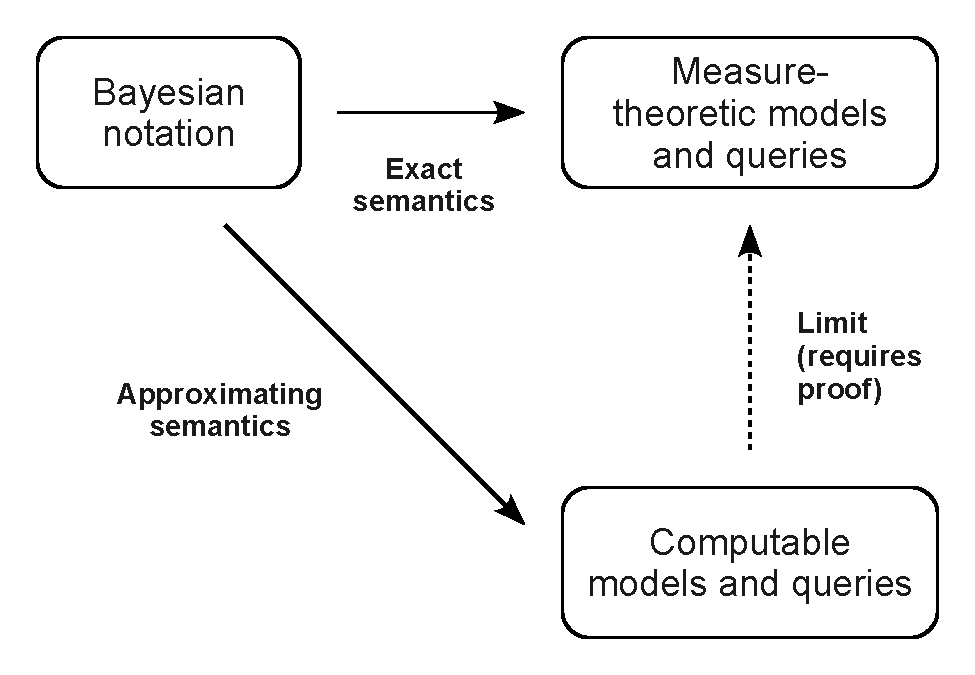
\includegraphics[width=4.0in]{figures/semantics.pdf}
\caption[ ]{An informal commutative diagram showing, as arrows, what is necessary for a Bayesian modeling and inference language to be trustworthy. ``Limit'' means that as an approximating program's output approaches a value, it approaches the value specified by the exact semantics.}
\label{figure:my-job}
\end{figure*}

As Figure~\ref{figure:my-job} illustrates, the solution requires both an exact and an approximating semantics. Only the approximating semantics is meant to be implemented. Its output is parameterized on the closeness of its approximation. (For example, if it represents a sampling method, it could be parameterized on the number of samples.) If the approximations provably converge to the exact answers, the language is trustworthy. We might say that it is ``trustworthy in the limit.''

Therefore, a trustworthy language for Bayesian modeling and inference is defined by
\begin{itemize}
	\item An exact semantics (to provide a standard for the approximating semantics).
	\item An approximating semantics (to provide a standard for implementations).
	\item A proof that computable approximations converge to the exact.
\end{itemize}
Ideally, the approximating semantics is derived from the exact, and convergence is by construction.

It is perhaps natural to ask why we should not draw the ``limit'' arrow in Figure~\ref{figure:my-job} from ``computable models and queries'' back to ``Bayesian notation.'' But the question is misguided. Bayesian notation is just syntax: it describes a thing, but is not the thing itself.

It makes more sense to ask why we should not point the ``limit'' arrow at some class of Bayesian models. The answer is that models that Bayesians reason with, which consist of mass and densitity functions, summation, and a usually unspecified kind of integration, cannot explain enough theories. Example~\ref{example:no-density} defines a simple, sensible random variable whose distribution has no Bayesian model. We might try to hack one together using some combination of mass and density functions, but we would lose our certainty that the model is correct. Hacking a model together becomes impossible when we consider infinite theories, in which the joint density of any outcome would be zero.

\subsection*{Useful}

We generally think of languages as being \keyword{useful} when they save us time by automating our calculations. While important, this is only one aspect of a language's usefulness. In addition, a language might be useful if it
\begin{itemize}
	\item Allows us to express our ideas and reason about them precisely.
	\item Provides abstraction mechanisms, such as functions or classes, so that we can do so at arbitrarily high levels.
\end{itemize}

According to this criteria, having just an exact semantics for constructive Bayesian notation is useful. When defining a probabilistic theory in prose, it is easy to do so in a way that is ambiguous, contradictory, or unfaithful to the laws of probability. Writing it so that it can be mechanically interpreted as a measure-theoretic model erases all of these concerns.

Also, besides notation for sequencing and specialized languages like probabilistic context-free grammars, Bayesian notation has no real abstraction mechanisms. It is currently very difficult to formalize ``we model this phenomenon using a probabilistic context-free grammar, but with certain cross-links.'' With the right abstractions it could be expressed naturally as recursion or corecursion.

However, we cannot downplay the importance of automating calculations. Therefore, in this investigation, a useful language must also have at least one implementation. Implementations should be able to compute or approximate most interesting queries.

To be useful, a language that includes existing notation must meet an additional criterion: the interpretation of existing notation must be correct. As a counterexample, consider a semantics that interprets ``$X \sim \Normal(0,1)$'' as a command to launch nuclear missiles at the user's house.

A less obviously incorrect semantics might interpret ``$X \sim \Normal(0,1)$'' as stating that $X$'s distribution is approximately Normal over 64-bit floating-point values as defined in IEEE 754-2008. This interpretation is wrong because Bayesians intend for $X$ to have a specific density over $\Re$. Or a semantics might transform
\begin{equation}
\begin{aligned}
	X &\sim \Normal(0,1) \\
	Y &\sim \Normal(0,1)
\end{aligned}
\end{equation}
into $X \sim \Normal(0,1);\ Y := X$ before fully interpreting it. This interpretation not only disregards the implied independence of $X$ and $Y$, but makes them as dependent as possible.

As much of the often-fuzzy notion of ``correctness'' as can be formalized should be collected into a theorem stating semantic intent, and proved. The rest should be reasonably demonstrated. In a language for constructive modeling and inference, as the floating-point example shows, semantic intent must be a property of the exact semantics.

\section{Proof and Supporting Evidence}

\paragraph{Semantics.} Blah blah blah.

Blah.

\paragraph{Properties.} Blah blah blah.

Blah.

\paragraph{Test Cases.} Blah blah blah.

Blah.
\end{comment}
